
\subsection{Referencia de tensión basada en el \textit{TL431}}

\label{section:voltage_reference}


\begin{wrapfigure}{rH}{0.18\textwidth}
\begin{center}
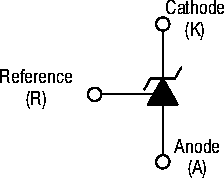
\includegraphics[width=0.15 \textwidth, angle=0]{./img/voltage_reference/reference0.png}
\end{center}
\caption{\label{fig:fig_vref_cir_0}\footnotesize{$TL431$}}
\end{wrapfigure}


Se debe analizar un circuito de referencia de tensión, basado en la referencia integrada $TL431$, el cual se trata de un regulador paralelo (shunt regulator) programable, que opera básicamente como un zener configurable, (su símbolo es similar, como se muestra en la figura~\figref{fig:fig_vref_cir_0}), de bajo coeficiente térmico y bajo ruido, puede ser configurado para tensiones de salida desde el valor de la referencia interna, $V_{ref} = 2.5 \si[per-mode=symbol]{\volt}$, hasta $36 \si[per-mode=symbol]{\volt}$, no tiene un valor per se de tensión de \quotemarks{dropout}, pero por supuesto es necesario que la tensión de entrada sea mayor que la de salida, al tiempo que es polarizado con una corriente de al menos $1 \si[per-mode=symbol]{\milli\ampere}$, lo que impone indirectamente el valor mínimo de tensión de entrada.
La referencia tiene capacidad de absorber desde $1 \si[per-mode=symbol]{\milli\ampere}$ a $100 \si[per-mode=symbol]{\milli\ampere}$ y tiene típicamente una impedancia dinámica de $220 \si[per-mode=symbol]{\milli\ohm}$. La referencia interna de tensión es del tipo \quotemarks{bandgap reference}, que como se explica en el libro G\&M~\cite{Gray_Meyer5}, logra una tensión independiente de la temperatura. Si se tiene en cuenta el esquema simplificado del circuito proveído por el fabricante, que se puede ver el la figura~\figref{fig:fig_vref_cir_2}, se hace mas simple ver la estructura del circuito que se propone analizar, el mismo se puede ver en la figura~\figref{fig:fig_vref_cir_1}. La estructura corresponde al de una fuente de tensión regulada realimentada serie, el elemento de paso es el transistor, $Q_{1}$ en ese diagrama, los resistores, $R_{1}$ y $R_{2}$, son la red de realimentación, que muestrean la tensión de salida y el amplificador suma (resta) en la entrada, teniéndose realimentación del tipo \textbf{serie-paralelo}, que estabiliza la ganancia de tensión, el resistor $R_{3}$ es el que provee la corriente de polarización al $TL431$ y $R_{4}$ está limitando la corriente de colector máxima que puede circular por $Q_{1}$. Interpretado de esta manera es fácil deducir la expresión de cálculo que el fabricante provee para la tensión de salida, ya que, asumiendo que la ganancia del amplificador interno es lo suficientemente elevada como para que la ganancia de lazo sea mucho mayor a $1$, sabemos que la ganancia a lazo cerrado será $\frac{1}{f}$, y es fácil ver que se tiene $f = \frac{R_{2}}{R_{1} + R_{2}}$, por lo tanto la salida que se tendrá será $V_{o} = V_{ref} \cdot \left(1 +  \frac{R_{1}}{R_{2}} \right)$, que salvo por la corrección por la corriente que toma el amplificador, coincide con la proveída. Queda el capacitor $C_{1}$, este se encuentra conectado de manera de proveer realimentación del tipo \textbf{paralelo-paralelo}, de un valor creciente con la frecuencia, de modo que está cumpliendo una función de compensación, lo cual era esperable dado que se tiene internamente un amplificador realimentado. Nuestro circuito tendrá una mayor capacidad de manejar corriente, gracias al transistor $Q_{1}$, que al ser un $BD135$, tiene un $\beta$ mínimo de 25, con lo que tomará $25$ veces menos corriente por la base, se espera que el transistor mejore la resistencia dinámica del $TL431$, ya que se tendrá aproximadamente $r_{d}$ del transistor dividida por la ganancia de lazo, se realizó una simulación con el comando \textbf{SPICE} \textit{.ac}, usando una fuente de corriente de señal a la salida del circuito, para obtener la impedancia de salida, se obtuvo para este circuito $11 \si[per-mode=symbol]{\milli\ohm}$.
El modelo que provee el fabricante es un macro-modelo, que por supuesto no simula todos los detalles del comportamiento, en particular la hojas de datos especifica que la mínima corriente de cátodo para regulaciión es minimamente $1 \si[per-mode=symbol]{\milli\ampere}$ y típicamente $500 \si[per-mode=symbol]{\micro\ampere}$, sin embargo la simulación muestra que regula con corrientes mucho menores, por lo tanto para determinar la máxima corriente que el circuito puede entregar se todo el valor mínimo de corriente de cátodo, $500 \si[per-mode=symbol]{\micro\ampere}$, como limitante y se determinó un valor de corriente de salida, tal que provoque que la base del transistor tome una corriente tal que lleve la de cátodo a ese valor, y se obtuvo $50.4 \si[per-mode=symbol]{\milli\ampere}$.La estabilidad con la temperatura del circuito debería ser similar a la del $TL431$, que es de $40 ppm/^{\circ}C$.



\begin{figure}[H] %htb
\begin{center}
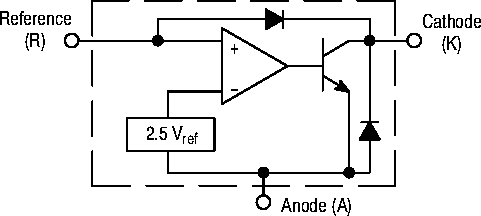
\includegraphics[width=0.65 \textwidth, angle=0]{./img/voltage_reference/reference2.png}
\end{center}
\caption{\label{fig:fig_vref_cir_2}\footnotesize{Esquema interno simplificado del $TL431$}}
\end{figure}



\begin{figure}[H] %htb
\begin{center}
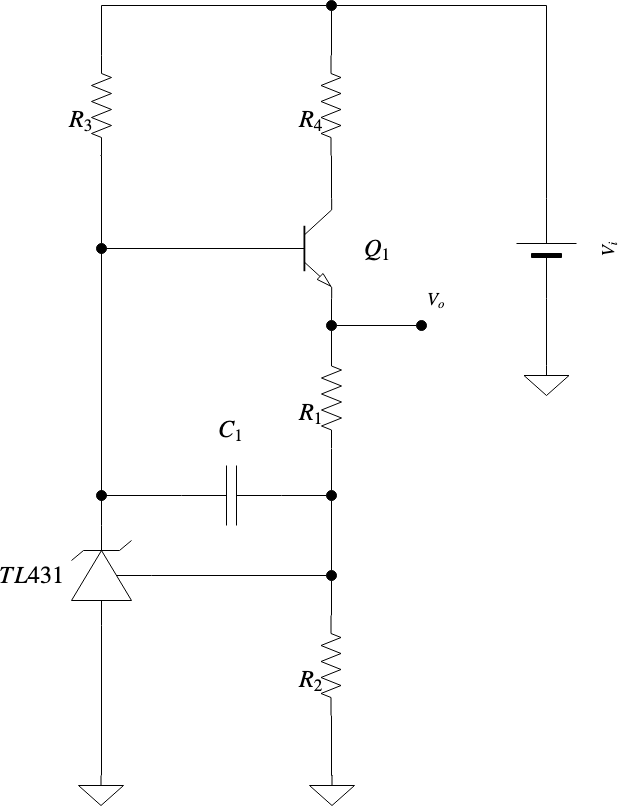
\includegraphics[width=0.50 \textwidth, angle=0]{./img/voltage_reference/reference1.png}
\caption{\label{fig:fig_vref_cir_1}\footnotesize{Circuito de referencia de tensión analizado}}
\end{center}
\end{figure}



\clearpage